
\documentclass[11pt]{article}

% DEFAULT PACKAGE SETUP

\usepackage{setspace,graphicx,epstopdf,amsmath,amsfonts,amssymb,amsthm,versionPO}
\usepackage{marginnote,datetime,enumitem,subfigure,rotating,fancyvrb}
\usepackage{hyperref,float}
\usepackage[longnamesfirst]{natbib}
\usdate

% These next lines allow including or excluding different versions of text
% using versionPO.sty

\excludeversion{notes}		% Include notes?
\includeversion{links}          % Turn hyperlinks on?

% Turn off hyperlinking if links is excluded
\iflinks{}{\hypersetup{draft=true}}

% Notes options
\ifnotes{%
\usepackage[margin=1in,paperwidth=10in,right=2.5in]{geometry}%
\usepackage[textwidth=1.4in,shadow,colorinlistoftodos]{todonotes}%
}{%
\usepackage[margin=1in]{geometry}%
\usepackage[disable]{todonotes}%
}

% Allow todonotes inside footnotes without blowing up LaTeX
% Next command works but now notes can overlap. Instead, we'll define 
% a special footnote note command that performs this redefinition.
%\renewcommand{\marginpar}{\marginnote}%

% Save original definition of \marginpar
\let\oldmarginpar\marginpar

% Workaround for todonotes problem with natbib (To Do list title comes out wrong)
\makeatletter\let\chapter\@undefined\makeatother % Undefine \chapter for todonotes

% Define note commands
\newcommand{\smalltodo}[2][] {\todo[caption={#2}, size=\scriptsize, fancyline, #1] {\begin{spacing}{.5}#2\end{spacing}}}
\newcommand{\rhs}[2][]{\smalltodo[color=green!30,#1]{{\bf RS:} #2}}
\newcommand{\rhsnolist}[2][]{\smalltodo[nolist,color=green!30,#1]{{\bf RS:} #2}}
\newcommand{\rhsfn}[2][]{%  To be used in footnotes (and in floats)
\renewcommand{\marginpar}{\marginnote}%
\smalltodo[color=green!30,#1]{{\bf RS:} #2}%
\renewcommand{\marginpar}{\oldmarginpar}}
%\newcommand{\textnote}[1]{\ifnotes{{\noindent\color{red}#1}}{}}
\newcommand{\textnote}[1]{\ifnotes{{\colorbox{yellow}{{\color{red}#1}}}}{}}

% Command to start a new page, starting on odd-numbered page if twoside option 
% is selected above
\newcommand{\clearRHS}{\clearpage\thispagestyle{empty}\cleardoublepage\thispagestyle{plain}}

% Number paragraphs and subparagraphs and include them in TOC
\setcounter{tocdepth}{2}

% JF-specific includes:

\usepackage{indentfirst} % Indent first sentence of a new section.
\usepackage{endnotes}    % Use endnotes instead of footnotes
\usepackage{jf}          % JF-specific formatting of sections, etc.
\usepackage[labelfont=bf,labelsep=period]{caption}   % Format figure captions
\captionsetup[table]{labelsep=none}

% Define theorem-like commands and a few random function names.
\newtheorem{condition}{CONDITION}
\newtheorem{corollary}{COROLLARY}
\newtheorem{proposition}{PROPOSITION}
\newtheorem{obs}{OBSERVATION}
\newcommand{\argmax}{\mathop{\rm arg\,max}}
\newcommand{\sign}{\mathop{\rm sign}}
\newcommand{\defeq}{\stackrel{\rm def}{=}}

\begin{document}

\setlist{noitemsep}  % Reduce space between list items (itemize, enumerate, etc.)
\onehalfspacing      % Use 1.5 spacing
% Use endnotes instead of footnotes - redefine \footnote command
\renewcommand{\footnote}{\endnote}  % Endnotes instead of footnotes

\title{Resource Reallocation with Carbon Emission Policies}
\author{Seyyed Morteza Aghajanzadeh}
\date{\today}

% Create title page with no page number

\maketitle
\thispagestyle{empty}

\bigskip

\centerline{\bf ABSTRACT}

\begin{doublespace}  % Double-space the abstract and don't indent it
  \noindent 
  Governments worldwide are implementing policies to mitigate carbon emissions, necessitating significant economic resource reallocation. This study investigates the economic consequences of these shifts, focusing on quantifying reallocation costs and delineating conditions for optimal resource distribution. Utilizing a model of a closed economy characterized by monopolistic competition and firm heterogeneity, the study distinguishes between 'green' (eco-friendly) and 'brown' (fossil fuel-dependent) capital in the production function. The emission function has been extended to incorporate variable parameters that reflect the environmental impacts of these resources. This analysis aims to provide critical insights into the dynamics of resource allocation under environmental policy constraints, underscoring the trade-offs between economic output and environmental sustainability. The results are intended to guide policymaking by clarifying the economic costs associated with transitioning to a low-carbon economy and outlining strategies to balance environmental and economic objectives optimally.
\end{doublespace}

\medskip

\noindent JEL classification: XXX, YYY.

\clearpage



\noindent In the face of escalating global environmental challenges, policymakers around the world have ramped up efforts to mitigate pollution and greenhouse gas emissions, deploying an arsenal of policy tools. These tools range from punitive measures like taxes or outright bans on environmentally detrimental investments, to incentives such as subsidies for adopting green technologies. Such policy measures have fundamentally shifted the landscape of marginal costs for businesses, compelling them to reevaluate their investment strategies. This policy-induced shift has catalyzed a movement towards new equilibriums, characterized by lower emission levels and a heightened focus on sustainable practices. However, this transition is not without its economic ramifications, as it entails not only shifts in corporate investment strategies but also significant economic reallocation and potential inefficiencies. These developments underscore the importance of scrutinizing the efficiency and economic ramifications of environmental policies, prompting a reevaluation of how effectively resources and inputs are allocated in this new context.

Building on the seminal research by \cite{whited2021misallocation} and\cite{hsieh2009misallocation}, which explores the adverse effects of resource misallocation on the economy's overall efficiency, this paper extends the conversation to the environmental policy. Misallocation, in essence, refers to a scenario where resources are not optimally distributed among firms, leading to suboptimal production outcomes. In the context of environmental policy, such misallocation is seen as a strategic reconfiguration of resources among firms, spurred by policy-induced shifts in their marginal costs. This dynamic, while aimed at encouraging more sustainable practices, introduces complexities in assessing the real economic impact of environmental policies. It raises pertinent questions about the trade-offs between economic efficiency and environmental sustainability, making it a fertile ground for inquiry.

To navigate these complexities, my model introduces novel elements to the \cite{hsieh2009misallocation}, starting with a critical distinction between 'brown' and 'green' capital. 'Brown' capital, characterized by its reliance on fossil fuels and its significant environmental footprint, contrasts sharply with 'green' capital, which embodies renewable and environmentally benign resources. This distinction is more than mere semantics; it acknowledges the heterogeneous impact of different types of capital on production and the environment. By moving beyond the traditional, homogenized view of capital, the model illuminates the nuanced roles these capital forms play in economic productivity and environmental sustainability. Furthermore, the introduction of a pollution function represents a significant leap forward. This function quantitatively links the utilization of brown and green capitals in production processes to their respective environmental impacts, enabling a detailed analysis of how production decisions affect ecological outcomes. This analytical enhancement allows the model to capture the complex interplay between economic activities and environmental health, offering insights into how shifts towards greener capital can mitigate environmental damage while fostering economic resilience.

To empirically anchor this theoretical exploration, I employ comprehensive registry data from a wide array of Swedish corporations, encompassing both publicly listed and privately held entities. Sweden's forefront position in enacting and enforcing some of the most stringent environmental regulations globally offers a unique vantage point to examine the economic repercussions of such policies. By meticulously analyzing this data, I aim to quantify the model's parameters and assess the extent and nature of economic reallocation in response to environmental policies. This empirical strategy not only validates the theoretical model but also provides a concrete basis for evaluating the efficacy and economic impacts of environmental regulations. Ultimately, this research endeavors to illuminate the pathways through which environmental policies can be calibrated to balance economic efficiency with the imperative of environmental sustainability, thereby contributing to the ongoing dialogue on sustainable development.

\section{The Model} \label{sec:Model}

This section outlines my closed-economy model, characterized by heterogeneous firms operating under standard monopolistic competition. Drawing inspiration from \cite{hsieh2009misallocation}, I delve into the environmental and technological underpinnings of production, the intricacies of firm-level decision-making on inputs and pricing, and the broader implications of resource reallocation within the economy.

\subsection{Environment and Technology} \label{sec:env_tech}

Firms in the model produce a single good using labor and capital as inputs where there is two possible type of capital: Green and Brown. The production function of the firm is given by:
\begin{equation}
    \label{eq:firm_output}
    Y_{si} = \hat{A}_{si}\hat{K}_{si}^{\beta_s} L_{si}^{1-\beta_s}
    \quad,\qquad\hat{K} = (
        \alpha_s G_{si}^{\frac{\gamma_s-1}{\gamma_s}} + (1-\alpha_s) B_{si}^{\frac{\gamma_s-1}{\gamma_s}}
    ) ^ {\frac{\gamma_s}{\gamma_s-1}}
\end{equation}
Here $Y_{si}$ is the output of the firm $i$ in sector $s$ that use  labor ($L_{si}$) and an aggregate capital input ($\hat{K}_{si}$). The aggregate capital input, $\hat{K}_{si}$, is a function of Green capital ($G_{si}$) and Brown capital ($B_{si}$), showcasing the firm's capital composition. Key parameters in this function include $\alpha_s$, which reflects the share of green capital in total capital, indicating its critical role in the production capacity of the firm. The parameter $\beta_s$ represents the capital's contribution to the production process, highlighting the importance of capital input relative to labor. The elasticity of substitution between green and brown capital is denoted by $\gamma_s$, which measures the ease with which firms can switch between these two types of capital. Lastly, $\hat{A}_{si}$ represents the total factor productivity (TFP), indicating the overall efficiency of the firm in converting inputs into output.

Building upon the production framework, the model also accounts for pollution emissions as an inevitable by-product of the manufacturing process. This aspect introduces an environmental dimension, linking the firm's production choices to ecological impacts. The formulation for pollution emissions mirrors the structure of the production function but is specified with distinct parameters:
\begin{equation}
    \label{eq:firm_emission}
    E_{si} = \tilde{A}_{si}\tilde{K}_{si}^{\theta_s} L_{si}^{1-\theta_s} \quad,\qquad \tilde{K} = (
        \mu_s G_{si}^{\frac{\eta_s-1}{\eta_s}} + (1-\mu_s) B_{si}^{\frac{\eta_s-1}{\eta_s}}
    ) ^ {\frac{\eta_s}{\eta_s-1}}
\end{equation}
Within this framework, $E_{si}$ represents the emissions from firm $i$ in sector $s$, with $\tilde{K}{si}$ adjusting the capital input for emission calculations. The emission equation introduces $\mu_s$ to quantify the relative importance of green capital in mitigating emissions, reflecting a firm's commitment to environmental sustainability. The parameter $\theta_s$ captures the role of capital in emissions, analogous to its influence in the production process but focused on the environmental externality. The elasticity of substitution between green and brown capital, denoted by $\eta_s$, now portrays the firm's flexibility in shifting towards greener production methods to lower emissions. Lastly, $\tilde{A}{si}$, or emission productivity, measures how  a firm generates emissions, indicating variability in pollution levels across firms despite using the same technology within a sector. This dual approach to modeling production and emissions encapsulates the complex interplay between economic productivity and environmental impact, highlighting the heterogeneity in firm-level responses to ecological considerations.

Integrating sector-level production and emissions into the model adds another layer to our understanding of the economy's structure and its environmental impact. At the sector level, the model assumes that the combined output, $Y_s$, is derived from the individual outputs of firms within that sector, using a constant elasticity of substitution (CES) function. This approach is formalized as:
\begin{equation}
    Y_s = \left(
        \sum_{i=1}^I Y_{si}^{\frac{\sigma_s-1}{\sigma_s}}
    \right)^{\frac{\sigma_s}{\sigma_s-1}}
\end{equation}
Here, $\sigma_s$ represents the elasticity of substitution between products from different firms within the sector. A higher $\sigma_s$ implies greater substitutability among firms' outputs, facilitating competition and diversification in the sector.

Transitioning from the sectoral to the economy-wide perspective, the total output, $Y$, aggregates the sector outputs using a Cobb-Douglas function. This is represented as:
\begin{equation}
    Y = \Pi_1^S Y_s^{\lambda_s}, \quad \text{where} \quad \sum^S \lambda_s = 1
\end{equation}
In this formula, $\lambda_s$ denotes the weight of each sector's output in the economy, constrained by the condition that all sector weights sum up to one. This constraint ensures a balanced contribution of each sector to the economy, reflecting the diverse composition of economic activities.

However, the aggregation of emissions adopts a straightforward approach, summing up the emissions from all firms within a sector to determine sector emissions, $E_s$, and subsequently summing these across all sectors to calculate the economy's total emissions, $E$. The equations for aggregated emissions are presented as:
\begin{equation}\label{eq:sector_emission}
    E_s = \sum_{i=1}^I E_{si}, \quad E = \sum_{s=1}^S E_s
\end{equation}

This method highlights the cumulative environmental impact of production, emphasizing the direct link between economic activities and their ecological consequences. By modeling both production and emissions at the firm, sector, and economy levels, the framework provides a comprehensive view of the trade-offs between economic development and environmental sustainability.



\subsection{Optimal Allocation} \label{sec:optimal_allocation}

When delving into the firm's decision-making process concerning input selection and pricing to optimize profit, it becomes essential to consider the costs associated with labor, green capital, and brown capital. Each of these inputs incurs specific costs: $w_{si}$ for labor, $r_{si}^G$ for green capital, and $r_{si}^B$ for brown capital. However, the model introduces an additional layer of complexity by incorporating market frictions, which are influenced by rising social concerns around Environmental, Social, and Governance (ESG) issues. These frictions, represented by $\tau_{G}$ for green capital, $\tau_{B}$ for brown capital, $\tau_{L}$ for labor, and $\tau_{P}$ for the product market, can either increase costs (when positive, indicating an added charge) or decrease them (when negative, indicating a subsidy). Furthermore, firms are required to pay a sector-wide emission tax, denoted by $\tau_{E}$.

Given these factors, the profit equation for a firm can be structured as follows:
\begin{equation}
    \pi_{si} = (1+\tau_{s}^p) P_{s} Y_{s} - \left(\left[
        (1+ \tau_{G_{s}}) r_{si}G_{si} + (1+ \tau_{B_{s}}) r_{si}B_{si} + (1+ \tau_{l_{s}}) w_{si}l_{si}
    \right] + {\tau_{E} E_{si}}\right)
\end{equation}

Here, the profit, $\pi_{si}$, is derived from the revenue (the product of the output price, $P_{si}$, and quantity, $Y_{si}$, adjusted for product market friction, $\tau_{si}^P$) minus the costs associated with inputs, taxes, and frictions. The cost term encapsulates expenses for labor, both types of capital, the emission tax, and any additional market frictions that the firm encounters. This model thus accounts for a range of economic and social factors influencing firm behavior, reflecting the complex interplay between profitability, market conditions, and societal expectations.

To maximize the profit, a firm must strategically determine its input mix before setting the price of its product. This process begins with minimizing the cost of production for a predetermined output level, denoted as $\bar{Y}_{si}$. The optimal mix of inputs—specifically, the balance between green and brown capital, as well as the proportion of labor used—is critical in achieving cost efficiency(Check Appendix~\ref{Ap:optimal level for given output} for the proof).
\begin{equation}\label{eq:capital_optimal_ratio}
  z^k_{si} \equiv \frac{G_{si}}{B_{si}} = \left[
    \frac{\alpha_s}{1-\alpha_s} \dfrac{\frac{\partial }{\partial B}Cost_{si}}{\frac{\partial }{\partial G}Cost_{si}}
\right] ^ {\gamma_s} 
\end{equation}
This equation reflects the firm's preference for green over brown capital, influenced by the parameter $\alpha_s$, which indicates the importance of green capital in production. The ratio of marginal costs ($\frac{\partial Cost_{si}}{\partial B}/\frac{\partial Cost_{si}}{\partial G}$) adjusts the balance, taking into account the cost implications of each type of capital. The elasticity of substitution between green and brown capital, $\gamma_s$, further modifies this ratio, determining the firm's flexibility in substituting between the two capitals.

For labor relative to the combined capital input ($\hat{K}{si}$), the optimal ratio ($z^l{si}$) is given by:
\begin{equation}\label{eq:labor_optimal_ratio}
  \begin{split}
    z^l_{si} \equiv \frac{L_{si}}{\hat{K}_{si}} & = \frac{1-\beta_s}{\beta_s} \frac{1}{1-\alpha_s} (\alpha_s {z^k_{si}}^{(\gamma_s -1)} + (1-\alpha_s))^{\frac{1}{1-\gamma_s}}\dfrac{\frac{\partial }{\partial B}Cost_{si}}{\frac{\partial }{\partial L}Cost_{si}}\\
    & = \frac{1-\beta_s}{\beta_s} \frac{1}{\alpha_s}(\alpha_s  + (1-\alpha_s){z^k_{si}}^{(1-\gamma_s )})^{\frac{1}{1-\gamma_s}}\dfrac{\frac{\partial }{\partial G}Cost_{si}}{\frac{\partial }{\partial L}Cost_{si}}
\end{split}
\end{equation}
This equation integrates the capital-to-labor ratio within the production function, factoring in the importance of capital ($\beta_s$) and the predetermined optimal capital mix ($z^k_{si}$). The terms involving partial derivatives of costs with respect to labor and capital inputs adjust the ratio based on the relative cost efficiency of labor and capital.

In essence, these equations guide the firm in adjusting its input mix to minimize production costs effectively, taking into account the price and efficiency of labor and capital, as well as market and environmental constraints. This analytical foundation enables a firm to optimize its production inputs before determining the optimal pricing strategy to maximize profit.

The connection between firm output and emissions is explicitly considered, revealing the environmental consequences of production activities. The mathematical expression for the optimal level of emissions, which incorporates various factors including the firm's choice of inputs and its output level, is presented as follows:
\begin{equation}
    E_{si} = {\frac{\tilde{A}_{si}}{\hat{A}_{si}}(\frac{\phi_{si}}{z^{l}_{si}})^{\theta_s} {z^{l}_{si}}^{\beta_s}} \bar{Y}_{si} = \psi_{si}\bar{Y}_{si}, \quad \text{where} \quad \phi_{si}  = \frac{(\mu_s  + (1-\mu_s){z^k_{si}}^{(1-\eta_s )})^ {\frac{\eta_s}{\eta_s-1}}}{(\alpha_s  + (1-\alpha_s){z^k_{si}}^{(1-\gamma_s )}) ^{\frac{\gamma_s}{\gamma_s-1}}} 
\end{equation}
This equation, detailed in Appendix~\ref{Ap:optimal emission level}, outlines the linear relationship between emissions ($E_{si}$) and the firm's output ($\bar{Y}{si}$). The coefficient $\frac{\tilde{A}{si}}{\hat{A}{si}}$ captures the relative efficiency of production in terms of emissions, with $\tilde{A}{si}$ and $\hat{A}{si}$ representing emission productivity and total factor productivity, respectively. The term $\phi{si}$, an adjustment factor, integrates the environmental effects of the chosen capital mix through parameters such as $\mu_s$ (the importance of green capital), $\eta_s$ (the elasticity of substitution between green and brown capital), and the optimal capital ratio $z^k_{si}$. This formulation highlights how a firm's input decisions—specifically, the balance between green and brown capital and the labor-to-capital ratio ($z^l_{si}$)—affect its emissions, thereby linking economic decisions to their environmental impacts.\footnote{
  I can use the same notation and drive the emission to sale ratio by using the fact that $\nu_s$ is normalized to 1. This can be done:
  \begin{equation*}
    \frac{E_{si}}{(P_{si}Y_{si})^{\frac{\sigma_s}{\sigma_s-1}}} = \frac{\psi_{si}}{\nu_s} = \psi_{si} 
  \end{equation*}
}



After determining the optimal mix of inputs for production, a firm set the price of its product to maximize profit. This decision-making process involves calculating the optimal price, which, as delineated in Appendix~\ref{Ap:optimal price}, follows a specific formula:
\begin{equation}
    \begin{split}
         P_{si} =& \frac{1}{1+\tau_{si}^p}\frac{\sigma_s}{\sigma_s - 1} C_{si} \\
    \end{split}
\end{equation}

This equation illustrates that the optimal pricing strategy for a firm involves setting a price that exceeds its marginal cost, $C_{si}$, by a markup. The magnitude of this markup is determined by the elasticity of substitution, $\sigma_s$, between the products in the sector. Specifically, the term $\frac{\sigma_s}{\sigma_s - 1}$ represents the markup factor, which is inversely related to the elasticity; a higher elasticity (indicating products are more substitutable) leads to a lower markup. The adjustment factor $\frac{1}{1+\tau_{si}^p}$ accounts for any product market frictions, denoted by $\tau_{si}^p$, which could be due to taxes, subsidies, or other market conditions affecting the final price.

\subsection{Calibration} \label{sec:Calibration}
With the theoretical framework, I proceed to calibrate its parameters using the available summary statistics. Calibration is vital as it aligns the model with empirical data, thus boosting its predictive accuracy and practical relevance.

To initiate the calibration process, certain simplifying assumptions are necessary to effectively use the available data. Firstly, I assume that the emission function is solely influenced by brown capital, with $\theta_s = 1$ and $\mu_s = 0$. This assumption eliminates the need for estimating additional parameters, streamlining the calibration. Additionally, I presume there are no market frictions in the labor market ($\tau_L = 0$), product market ($\tau_P = 0$), green capital market ($\tau_G = 0$), and brown capital market ($\tau_B = 0$). These assumptions further reduce the complexity of the model by avoiding the estimation of extra parameters.

The goal is to replicate the findings in Table 2 from \cite{martinsson2024effect}, which presents results as ratios of optimal emission to optimal output. To achieve this, I assume a perfectly competitive market scenario, where the elasticity of substitution between products from different firms within the industry is infinite ($\sigma_s = \infty$). This assumption simplifies the model further, facilitating the use of the summary statistics provided.

Given these assumptions, I can rewrite the optimal emission level ratios as:
\input{model_elements/simplified model}

To align the model parameters with the provided summary statistics, I set $\beta_s$ to reflect the capital intensity at $0.6$. Considering the average annual wage in Sweden is $500,000$, I adjust the wage parameter, $w$, accordingly. The interest rate for capital is set at $11\%$, and I assume that there are no differences between the green and brown capital interest rates ($r_G=r_B = 11\%$).

The calibration still requires adjustment for four critical variables: $\alpha_s$, $\gamma_s$, $\tilde{A}{si}$, and $\hat{A}{si}$. I simulate the model across approximately 1200 firms, mirroring the firm count in \cite{martinsson2024effect}, all within the same sector but varying in productivity levels related to emissions and production ($\tilde{A}{si}$ and $\hat{A}{si}$). The productivity levels are drawn from a lognormal distribution.

Furthermore, to accurately represent the distribution as reported in \cite{martinsson2024effect}, I model firm-level workers using a lognormal distribution with a mean of 250 and a standard deviation of 900. Finally, to ensure the model accurately reflects the empirical data, the averages of $\hat{A}{si}$, $\tilde{A}{si}$, $\alpha_s$, and $\gamma_s$ are set to match the observed emission-to-sale ratio, total output, total emission, and the elasticity of the carbon tax on emission intensity as detailed in \cite{martinsson2024effect}.

In the model, the importance of green capital in the production function ($\alpha_s$) and the elasticity of substitution ($\gamma_s$) is critical, as illustrated in the subsequent figures. Figure~\ref{fig:production_emission} delineates the relationship between production and emissions, highlighting the role of parameters on the effectiveness of the policy. The calibration process is meticulously conducted to ensure that the model parameters not only resonate with the empirical evidence but also augment the model's predictive capabilities and enable a nuanced analysis of the benefits associated with resource reallocation.

\bigskip
\centerline{\bf [Place Figure~\ref{fig:production_emission} about here]}
\bigskip


Based on the explanation provided, $\alpha_s$ is set to \input{values/alpha estimate} and $\gamma_s$ to \input{values/gamma estimate} to align with the observed emission-to-sale ratio and the elasticity of the carbon tax on emission intensity as reported in \cite{martinsson2024effect}. To match the empirical data on total output, the average values of $\hat{A}{si}$ and $\tilde{A}{si}$ are set to \input{values/A hat estimate} and \input{values/A tilde estimate}, respectively.

One insightful approach is to evaluate three distinct environmental policies: a carbon tax, a green subsidy, and a brown tax. The green subsidy is implemented as a reduction in the interest rate on green capital, ranging from $0\%$ to $100\%$. Conversely, the brown tax is applied as an additional charge on the interest rate for brown capital, varying from $0\%$ to $400\%$. 

Using the calibrated model, I simulate the impact of these policies on the carbon intensity of the economy. The outcomes are illustrated in Figure~\ref{fig:intensity_tax_premium}, which displays the effects of each policy on reducing carbon intensity. It is evident from the results that the carbon tax and the brown capital tax are equivalent in terms of their impact on carbon intensity, while the green subsidy is more effective in lowering carbon intensity. 

\bigskip
\centerline{\bf [Place Figure~\ref{fig:intensity_tax_premium} about here]}

Furthermore, the model facilitates an analysis of these policies' effects on both production and emission levels within the economic framework. Figure~\ref{fig:emission_production} presents these dynamics, showing how the carbon tax and the brown capital tax curtail both production and emissions. Conversely, the green subsidy is associated with an augmentation in production levels without an increase in emissions. This analysis elucidates the complex interplay between environmental policies and economic activities, accentuating the inherent trade-offs between production efficiency and environmental sustainability. The combined implementation of a carbon tax and a green subsidy may offer an optimal strategy to balance these priorities, potentially enhancing economic productivity while concurrently mitigating emissions.

\bigskip
\centerline{\bf [Place Figure~\ref{fig:emission_production} about here]}

\subsection{Reallocation} \label{sec:reallocation}

To calculate the real gains from reallocation within the provided framework, I undertake a structured approach that leverages the model's theoretical foundation. This process involves several key steps, starting with the utilization of optimal input levels to ascertain the first-best output of each firm, and subsequently employing actual input levels to determine the actual output. By aggregating these outputs across firms within a sector, I can derive the economy-wide output under both optimal and actual scenarios. Comparing these outputs will then yield a measure of the real gains from reallocation, indicating the potential increase in efficiency and productivity through optimal resource distribution.

For the productivity expressions, the model delineates the production and emission productivity of a firm as functions of observable variables (Appendix~\ref{Ap:productivity} for the proof), except $\nu_s$, which represents a sector-specific constant that does not vary across firms. The productivity equations are given as follows, with a note that in subsequent analysis, $\nu_s$ will be normalized to 1 to simplify the computation:
\begin{equation}\label{eq:productivity}
  \hat{A}_{si} = \nu_s \dfrac{(P_{si}Y_{si})^{\frac{\sigma_s}{\sigma_s-1}}}{\hat{K}_{si}^{\beta_s} L_{si}^{1-\beta_s}}, \quad \text{where} \quad \nu_s = \frac{1}{P_s(P_sY_s)^{\frac{1}{\sigma_s-1}}}
\end{equation}
\begin{equation}\label{eq:emission_productivity}
  \tilde{A}_{si} = \dfrac{E_{si}}{\tilde{K}_{si}^{\theta_s} L_{si}^{1-\theta_s}}
\end{equation}
These equations incorporate a range of observable variables to model the production and emission efficiency of firms accurately. Although $\nu_s$ is not directly observable, its normalization does not affect the relative comparison of productivity across firms, allowing for a consistent analysis of reallocation benefits. This approach underscores the model's capability to bridge theoretical constructs with practical, observable metrics, facilitating an empirical assessment of productivity and environmental impact within the economic framework.

The final goalin optimizing resource allocation within an economy is to maximize output, which can be approached in two distinct manners depending on priorities: one method focuses on maximizing output without any emission constraints (Output Allocation), while the other incorporates these environmental constraints into the maximization process (Emission Allocation). Initially, in the absence of emission considerations, the strategy is to allocate resources—quantified as optimal amounts of green capital ($\hat{G}{si}$), brown capital ($\hat{B}{si}$), and labor ($\hat{L}{si}$), indicated by the hat notation—to fully maximize the productive potential of the economy. This pure output reallocation aims to enhance economic output to its highest feasible level by strategically deploying resources where they are most productive, without regard to the emissions generated in the process. Conversely, when environmental sustainability becomes a concurrent priority, the government seeks to balance the maximization of output with the goal of minimizing emissions. In this scenario, a different set of optimal resource levels—signified by the tilde notation ($\tilde{G}{si}$, $\tilde{B}{si}$, $\tilde{L}{si}$)—is determined to achieve a dual objective: pushing economic output towards its maximum while adhering to specified emission reduction targets. This nuanced approach to resource allocation underscores a commitment to both economic efficiency and environmental stewardship, illustrating a sophisticated strategy that aims to reconcile the often competing demands of maximizing output and minimizing environmental impact.

As outlined in Appendix~\ref{Ap:reallocation}, due to firms within a sector employing identical technology, the ratios of optimal inputs—green capital, brown capital, and labor—are consistent across these firms. This consistency in input ratios ensures that, regardless of individual firm characteristics, each entity adopts a proportionate mix of resources to maximize production efficiency.
\begin{gather}\label{eq:reallocation_firm_input_ratio}
    z_{s}^k = (\frac{\alpha_s}{1-\alpha_s})^{\gamma_s} \\
    z_{s}^l = \frac{1-\beta_s}{\beta_s} \frac{1}{1-\alpha_s} (\alpha_s {z^k_{s}}^{(\gamma_s -1)} + (1-\alpha_s))^{\frac{1}{1-\gamma_s}} \lambda_L
  \end{gather}

Upon establishing optimal input ratios, the sector's total resources are strategically distributed among firms. In scenarios prioritizing output reallocation, resources are allocated to the most productive firms, thereby optimizing sector-wide productivity by leveraging the capabilities of top performers. This approach ensures that firms with the highest productivity receive the lion's share of resources, maximizing overall economic output.
\begin{gather} \label{eq:output_allocation_allocation}
    \hat{L}_{si} = \dfrac{\hat{A}_{si}^{\sigma -1}}{\sum_j \hat{A}_{sj}^{\sigma -1}}L_s\\ 
    \hat{G}_{si} = \dfrac{\hat{A}_{si}^{\sigma -1}}{\sum_j \hat{A}_{sj}^{\sigma -1}}\dfrac{z_s^k}{1 + z_s^k} K_s\\ 
    \hat{B}_{si} = \dfrac{\hat{A}_{si}^{\sigma -1}}{\sum_j \hat{A}_{sj}^{\sigma -1}}\dfrac{1}{1 + z_s^k} K_s
\end{gather}

Conversely, emission reallocation takes a more nuanced approach by considering both productivity and environmental efficiency. Here, firms that strike the best balance between high productivity and low emissions are prioritized, receiving a larger allocation of resources. This strategy aims to marry economic efficiency with environmental stewardship, allocating resources to firms that contribute to a reduction in emissions without significantly sacrificing productivity.
\begin{gather} \label{eq:emission_allocation}
    \tilde{L}_{si} = \dfrac{\hat{A}_{si}^{\sigma -1}/\tilde{A}_{si}^{\sigma}}{\sum_j \hat{A}_{sj}^{\sigma -1}/ \tilde{A}_{sj}^{\sigma}}L_s\\
    \hat{G}_{si} = \dfrac{\hat{A}_{si}^{\sigma -1}/\tilde{A}_{si}^{\sigma}}{\sum_j \hat{A}_{sj}^{\sigma -1}/\tilde{A}_{sj}^{\sigma}}\dfrac{z_s^k}{1 + z_s^k} K_s\\ 
    \hat{B}_{si} = \dfrac{\hat{A}_{si}^{\sigma -1}/\tilde{A}_{si}^{\sigma}}{\sum_j \hat{A}_{sj}^{\sigma -1}/\tilde{A}_{sj}^{\sigma}}\dfrac{1}{1 + z_s^k} K_s
\end{gather}

These allocation strategies are underpinned by a sophisticated framework that considers the intricate balance between enhancing economic output and minimizing environmental impact. By meticulously allocating resources based on these criteria, the sector can achieve its dual goals of economic optimization and environmental sustainability.

Once I know the optimal resource allocation, the subsequent step involves computing the optimal output and emissions by substituting these ideal inputs into the respective formulas for firm output \eqref{eq:firm_output} and emissions \eqref{eq:firm_emission}. This calculation yields the theoretical maximum output and minimum emissions achievable under optimal conditions. By aggregating these optimal outputs and emissions across all firms within a sector, and subsequently for the entire economy, a comprehensive picture of potential economic efficiency and environmental impact under ideal resource distribution is formed. Comparing these aggregated optimal figures with the actual observed outputs and emissions allows for the quantification of the real gains from resource reallocation, highlighting the extent to which strategic redistribution can enhance economic productivity while minimizing environmental detriment. 

%% Calibration
\bigskip

\section{Data} \label{sec:Data}
Following the data compilation approach detailed by \cite{martinsson2024effect}, my dataset will be constructed. They created their dataset through the amalgamation of plant- and company-level registry details, covering aspects such as financial metrics, employee numbers, and sector categorizations, alongside CO2 emission records from 1990 to 2015. The Swedish Environmental Protection Agency (SEPA) furnished the CO2 emission data at both the plant and company levels, which includes emissions accounted for under the EU ETS. Registry information for both public and private Swedish firms was sourced from Upplysningscentralen (UC) for the period of 1990-1997 and Bisnode Serrano from 1998 to 2015.

The dataset I am creating will focus on company-level information, capturing data on the resources firms deploy, the outcomes they produce, and their environmental impact. This encompasses details such as capital and labor (as inputs); sales, and value addition (as outputs); and CO2 emissions (to gauge environmental impact). Additionally, the dataset will feature information on the industry sector, geographic location, and ownership structure of each company.

One challenge in constructing this dataset is the difficulty in distinguishing between green capital, which is environmentally beneficial, and brown capital, which has a detrimental environmental impact, due to the lack of direct indicators. To overcome this obstacle, I will use a proxy to identify green capital, with abatement costs serving as a viable option. This is based on the premise that abatement costs are indicative of investments in environmentally friendly capital.

Furthermore, integrating this dataset with bond market data could provide valuable insights, particularly in establishment of the relationship between green bonds and green capital. This linkage could be another proxy for green capital, as firms issuing green bonds are likely to have a higher proportion of green capital in their asset base. 

\section{Estimation} \label{sec:Estimation}
To calculate the parameter $\gamma_s$, indicative of the elasticity of substitution between capital and labor within sectors, a modified approach derived from the methodology presented in \cite{kmenta1967estimation} is employed. This method is specifically designed for estimating CES production functions, avoiding the direct use of structural assumptions from the model described in Section~\ref{sec:Model}. This choice is made to circumvent the theoretical scenario where an absence of financial restrictions, and hence no wedges, is assumed. Instead, this estimation method capitalizes on a different aspect of data variability than that used for determining wedge estimates, focusing on sector-level variations in the ratios of inputs to productivity.

In a hypothetical frictionless environment, one would not expect to find any correlation between these ratios and productivity levels, a situation that, according to \cite{kmenta1967estimation}, would imply an infinite elasticity of substitution. However, the presence of financial or environmental frictions introduces a tangible correlation between these variables, signifying a finite elasticity. Thus, the estimation of $\gamma_s$ serves to quantify the extent to which such frictions are uniformly present across firms within a sector, offering insights into average sector-specific variations in input ratios and productivity levels without pinpointing individual firm-level frictions.

As mentioned in Appendix~\ref{Ap:estimation}, the methodology for estimating the elasticity parameter $\gamma_s$ involves an ordinary least squares (OLS) analysis that incorporates firm-specific fixed effects. This approach is based on a regression derived from the first-order approximation of the production function at $\gamma_s = 1$, following the guidelines set by \cite{kmenta1967estimation}. An important aspect of this model is the nature of the error term, which is attributed to the variable $A_{si}$, indicative of the firm-specific productivity levels that are inherently correlated with the inputs. The identification of our model, particularly with the inclusion of fixed effects, is contingent upon the critical assumption that $A_{si}$'s variation is ob the firm level, manifesting without temporal fluctuations. This assumption is important for the robustness and validity of the OLS analysis, ensuring that the estimated $\gamma_s$ reflects the intrinsic elasticity of substitution between capital and labor, devoid of confounding temporal effects.

Exploring an alternative identification approach hinges on the premise that $A_{si}$, the firm-specific productivity term, follows an autoregressive pattern. This consideration allows for the application of a refined estimation strategy that employs quasi-differencing and the use of lagged instruments. This methodology draws inspiration from techniques similar to those outlined in \cite{blundell2000gmm} and \cite{davis2014macroeconomic}, offering a nuanced approach to capturing the dynamic aspects of productivity within firms.\footnote{
This alternative approach aligns with established strategies for production function estimation as seen in studies like \cite{olley1992dynamics}, \cite{levinsohn2003estimating}, and \cite{ackerberg2015identification}, underscoring the diversity of econometric methods tailored to understanding productivity dynamics.
} The potential challenges associated with employing the Generalized Method of Moments (GMM) in small samples, coupled with the size limitations of my industry-specific dataset, necessitate a cautious application of this method. Consequently, while the Ordinary Least Squares (OLS) method is utilized as the primary estimation technique, the GMM approach is also considered to verify the robustness of the results. This dual-method analysis ensures a comprehensive evaluation of the elasticity parameter $\gamma_s$, reinforcing the reliability of the conclusions drawn from the primary OLS estimation by corroborating them through an additional, albeit exploratory, GMM framework.





% To justify adding a subsection here, from now on, we'll assume
% \begin{condition}\label{cond:rates}
% $0 <  \hat{\mu} < \gamma\sigma^2$.
% \vspace{3mm}
% \end{condition}
% This condition might be useful if there was a model. 

% \subsection{Another Subsection, With a Figure}
% \label{sec:subsec}

% Figures get put at the end, with a note marking where they should go in the text, like this:

% \bigskip
% \centerline{\bf [Place Figure~\ref{fig:0} about here]}
% \bigskip

% \subsubsection{A Subsubsection with a Proposition}
% \label{sec:subsub}

% Let's put a proposition here.
% \begin{proposition} \label{prop:3}
% If Condition~\ref{cond:rates} is satisfied,  a solution to the central
% planner's problem, $V(B,D,t) \in C^2\left( {\mathbb R}_{+}^2 \times
%   [0,T] \right)$, with control $a:[0,1]\times[0,T]\rightarrow [-\lambda,\lambda]$
%  if  $\gamma>1$ is
% \begin{equation} \label{eq:valuea}
% V(B,D,t) =  - \frac{(B+D)^{1-\gamma}}{1-\gamma}   w\left(\frac{B}{B+D},t\right).
% \end{equation}
% \end{proposition}

%\clearpage

\appendix

\section{Definitions and Proofs} \label{Ap:defProof}
\subsection{Optimal input level for given output} \label{Ap:optimal level for given output}
\begin{equation*}
    \begin{split}
        \min_{GK_{si}, BK_{si}} & \quad
        \left[
        (1+ \tau_{G_{s}}) r_{si}G_{si} + (1+ \tau_{B_{s}}) r_{si}B_{si} + (1+ \tau_{l_{s}}) w_{si}l_{si}
    \right] + {\tau_{E} E_{si}} \\
        \text{s.t.} & \quad \hat{A}_{si}\hat{K}_{si}^{\beta_s} L_{si}^{1-\beta_s} = \bar{Y}_{si}\\
        % & \quad \tilde{A}_{si}\tilde{K}_{si}^{\theta_s} L_{si}^{1-\theta_s} = E_{si}
    \end{split}
\end{equation*}
\begin{equation*}
    \max  \quad
     - 		Cost \quad \text{s.t.} \quad \quad \hat{A}_{si}\hat{K}_{si}^{\beta_s} L_{si}^{1-\beta_s} = \bar{Y}_{si}
\end{equation*}
\begin{equation*}
z^k_{si} \equiv \frac{G_{si}}{B_{si}} = \left[
    \frac{\alpha_s}{1-\alpha_s} \dfrac{\frac{\partial }{\partial B}Cost_{si}}{\frac{\partial }{\partial G}Cost_{si}}
\right] ^ {\gamma_s} 
\end{equation*}
then we can rewrite the optimal capital level as:
\begin{equation*}
    \begin{split}
        \hat{K}_{si} &= B_{si}(\alpha_s {z^k_{si}}^{\frac{\gamma_s -1}{\gamma_s}} + (1-\alpha_s))^{\frac{\gamma_s}{\gamma_s - 1}}\\
        & = G_{si}(\alpha_s  + (1-\alpha_s){z^k_{si}}^{(1-\gamma_s )})^{\frac{\gamma_s}{\gamma_s - 1}}
    \end{split}
\end{equation*}
and then the optimal labor ratio is:
\begin{equation*}
    \begin{split}
    z^l_{si} \equiv \frac{L_{si}}{\hat{K}_{si}} & = \frac{1-\beta_s}{\beta_s} \frac{1}{1-\alpha_s} (\alpha_s {z^k_{si}}^{(\gamma_s -1)} + (1-\alpha_s))^{\frac{1}{1-\gamma_s}}\dfrac{\frac{\partial }{\partial B}Cost_{si}}{\frac{\partial }{\partial L}Cost_{si}}\\
    & = \frac{1-\beta_s}{\beta_s} \frac{1}{\alpha_s}(\alpha_s  + (1-\alpha_s){z^k_{si}}^{(1-\gamma_s )})^{\frac{1}{1-\gamma_s}}\dfrac{\frac{\partial }{\partial G}Cost_{si}}{\frac{\partial }{\partial L}Cost_{si}}
\end{split}
\end{equation*}
Let's define the use the optimal ratios ($z^k_{si} \equiv (\frac{G_{si}}{B_{si}})*$ and $z^l_{si} \equiv (\frac{L_{si}}{\hat{K}_{si}})^*$)
Optimal capital level for given output is 

\begin{equation*}
  \bar{Y}_{si} = \hat{A}_{si} \hat{K^*}_{si}^{\beta_s} {L^*}_{si}^{1-\beta_s} = \hat{A}_{si} \hat{K^*}_{si} ({\frac{L^*}{\hat{K^*}}})_{si}^{(1-\beta_s)}= \hat{A}_{si} \hat{K^*}_{si} {z_{si}^l}^{(1-\beta_s)}
\end{equation*}
we can rewrite the optimal capital level as:
\begin{equation*}
  \begin{split}
      \hat{K}_{si} &= B_{si}(\alpha_s {z^k_{si}}^{\frac{\gamma_s -1}{\gamma_s}} + (1-\alpha_s))^{\frac{\gamma_s}{\gamma_s - 1}}\\
      & = G_{si}(\alpha_s  + (1-\alpha_s){z^k_{si}}^{(1-\gamma_s )})^{\frac{\gamma_s}{\gamma_s - 1}}
  \end{split}
\end{equation*}
and then drive the optimal level of each type of capital:
\begin{equation*}
  G_{si}^* = \frac{\bar{Y}_{si}}{\hat{A}_{si}} \left(
        \alpha_s  + (1-\alpha_s){z^k_{si}}^{(1-\gamma_s )}
    \right)^{\frac{\gamma_s}{1-\gamma_s}} {z_{si}^l}^{(1-\beta_s)}
\end{equation*}
\begin{equation*}
  B_{si}^* = \frac{\bar{Y}_{si}}{\hat{A}_{si}} \left(\alpha_s {z^k_{si}}^{\frac{\gamma_s -1}{\gamma_s}} + (1-\alpha_s)
    \right)^{\frac{\gamma_s}{1-\gamma_s}} {z_{si}^l}^{(\beta_s-1)}
\end{equation*}
\begin{equation*}
  L_{si}^* = \frac{\bar{Y}_{si}}{\hat{A}_{si}}  {z_{si}^l}^{-\beta_s}
\end{equation*}
\subsection{Optimal Emission level for given output}\label{Ap:optimal emission level}
First we need to convert the production capital ($\hat{K}_{si}$) to the emission capital ($\tilde{K}_{si}$):
\begin{equation*}
    \begin{split}
        \tilde{K} = (
        \mu_s G_{si}^{\frac{\eta_s-1}{\eta_s}} + (1-\mu_s) B_{si}^{\frac{\eta_s-1}{\eta_s}}
    ) ^ {\frac{\eta_s}{\eta_s-1}} = G_{si}(\mu_s  + (1-\mu_s){z^k_{si}}^{(1-\eta_s )})^ {\frac{\eta_s}{\eta_s-1}}\\
    \hat{K} = (
        \alpha_s G_{si}^{\frac{\gamma_s-1}{\gamma_s}} + (1-\alpha_s) B_{si}^{\frac{\gamma_s-1}{\gamma_s}}
    ) ^ {\frac{\gamma_s}{\gamma_s-1}} = G_{si}(\alpha_s  + (1-\alpha_s){z^k_{si}}^{(1-\gamma_s )})^ {\frac{\gamma_s}{\gamma_s-1}}
    \end{split}
\end{equation*}
\begin{equation*}
    \Rightarrow \phi_{si} \equiv \frac{\tilde{K}}{\hat{K}} = \frac{(\mu_s  + (1-\mu_s){z^k_{si}}^{(1-\eta_s )})^ {\frac{\eta_s}{\eta_s-1}}}{(\alpha_s  + (1-\alpha_s){z^k_{si}}^{(1-\gamma_s )}) ^{\frac{\gamma_s}{\gamma_s-1}}} = \frac{(\mu_s {z^k_{si}}^{(\eta_s -1)}  + (1-\mu_s))^ {\frac{\eta_s}{\eta_s-1}}}{(\alpha_s {z^k_{si}}^{(\gamma_s -1)}  + (1-\alpha_s))^{\frac{\gamma_s}{\gamma_s-1}}}
\end{equation*}
As we can see the $\phi_{si}$ is a function of $z^k_{si}$, $\mu_s$, $\alpha_s$ and $\gamma_s$. Now we can calculate the optimal emission level ($E_{si}$) as follows:
\begin{equation*}
    \begin{split}
        E_{si} &= \tilde{A}_{si}\tilde{K}_{si}^{\theta_s} L_{si}^{1-\theta_s} = \tilde{A}_{si} \tilde{K}_{si} ({\frac{L_{si}}{\tilde{K}_{si}}})^{1-\theta_s}\\
    &= \tilde{A}_{si} (\phi_{si} \hat{K}_{si}) ({\frac{L_{si}}{\phi_{si} \hat{K}_{si}}})^{1-\theta_s}\\
    &= {\tilde{A}_{si}}{\phi_{si}}^{\theta_s} \hat{K}_{si} {z^{l}_{si}}^{1-\theta_s} \\
   & = {\tilde{A}_{si}}{\phi_{si}}^{\theta_s}{z^{l}_{si}}^{\beta_s-\theta_s}\hat{K}_{si}{z^{l}_{si}}^{1-\beta_s}\\
   & = \frac{\tilde{A}_{si}}{\hat{A}_{si}}(\frac{\phi_{si}}{z^{l}_{si}})^{\theta_s} {z^{l}_{si}}^{\beta_s} \bar{Y}_{si}
    \end{split}
\end{equation*}

\subsection{Optimal price}\label{Ap:optimal price}
We need to solve the firm price $P_{si}$ as function of sector price $P_s$, where $P_{si}$ is defined as the price of acquiring a unit of the firm benefit:
    \begin{gather*}
    \max_{P_{si}} \quad\pi_{si} =  (1+\tau_{si}^p)P_{si}Y_{si} - C_{si} {Y}_{si} \\
    \max  \quad (1+\tau_{si}^p)P_{si}( \frac{P_s}{ P_{si}})^{\sigma_s}{Y}_s - C_{si} (\frac{P_s}{ P_{si}})^{\sigma_s}{Y}_s \\
    \max \quad  (1+\tau_{si}^p)P_{si}^{1-\sigma_s}P_s^{\sigma_s}{Y}_s - C_{si} P_{si}^{-\sigma_s}P_s^{\sigma_s}{Y}_s \\
    \max \quad P_s^{\sigma_s}{Y}_s \left(
        (1+\tau_{si}^p)P_{si}^{1-\sigma_s} - C_{si} P_{si}^{-\sigma_s} 
    \right)\\
    \max \quad  (1+\tau_{si}^p)P_{si}^{1-\sigma_s} - C_{si} P_{si}^{-\sigma_s} \\
    \Rightarrow 0 = P_{si}^{-\sigma_s - 1} \left[
        (1+\tau_{si}^p)(1-\sigma_s)P_{si} + \sigma_s C_{si} 
    \right]
    \\
    \Rightarrow P_{si} = \frac{1}{1+\tau_{si}^p}\frac{\sigma_s}{\sigma_s - 1} C_{si} 
\end{gather*}
\subsection{Productivity of the firm}\label{Ap:productivity}

\begin{gather*}
    P_{si}^{\sigma_s} = P_s^{\sigma_s} Y_s Y_{si}^{-1} 
    \Rightarrow (P_{si}Y_{si})^{\sigma_s} = P_s^{\sigma_s} Y_s Y_{si}^{\sigma_s-1}
    \Rightarrow (P_{si}Y_{si})^{\sigma_s} = (P_sY_s)(P_sY_{si})^{\sigma_s-1}\\
    \Rightarrow (P_{si}Y_{si})^{\frac{\sigma_s}{\sigma_s-1}} = (P_sY_s)^{\frac{1}{\sigma_s-1}}P_sY_{si}\\
    \Rightarrow Y_{si} = \dfrac{(P_{si}Y_{si})^{\frac{\sigma_s}{\sigma_s-1}}}{P_s(P_sY_s)^{\frac{1}{\sigma_s-1}}}\\
    \Rightarrow \hat{A}_{si} = \frac{1}{P_s(P_sY_s)^{\frac{1}{\sigma_s-1}}}\dfrac{(P_{si}Y_{si})^{\frac{\sigma_s}{\sigma_s-1}}}{\hat{K}_{si}^{\beta_s} L_{si}^{1-\beta_s}} = \nu_s \dfrac{(P_{si}Y_{si})^{\frac{\sigma_s}{\sigma_s-1}}}{\hat{K}_{si}^{\beta_s} L_{si}^{1-\beta_s}}
\end{gather*}

\begin{gather*}
    E_{si} = \tilde{A}_{si}\tilde{K}_{si}^{\theta_s} L_{si}^{1-\theta_s} \Rightarrow \tilde{A}_{si} = \dfrac{E_{si}}{\tilde{K}_{si}^{\theta_s} L_{si}^{1-\theta_s}}\\
\end{gather*}

\subsection{Reallocation} \label{Ap:reallocation}


It is the social planner's problem to reallocate resources, therefore there is no need to price the inputs. The social planner's problem is to maximize the total real output subject to the resource constraint. Firms in the economy will produce the optimal level of output given the zero cost of inputs. The social planner's problem is:
\input{model_elements/social planner's problem}

Now I will write the lagrangian for the social planner's problem. The social planner's problem is to maximize the total output in the economy subject to the resource constraint. The lagrangian is:
\input{model_elements/social planner's problem - largranian}
where $\lambda_L$, $\lambda_E$ are the lagrange multipliers for the labor and emission constraints, respectively that are normalized by the capital lagrange multiplier. This results in the fact that the relative marginal cost of labor is $\lambda_L$ and the relative marginal cost of acquiring one unit of capital is 1. Now I can use the results from the firm's problem and the optimal input ratios to derive the optimal output and emissions for the social planner. The optimal input ratios are:
\begin{gather}\label{eq:reallocation_firm_input_ratio}
    z_{s}^k = (\frac{\alpha_s}{1-\alpha_s})^{\gamma_s} \\
    z_{s}^l = \frac{1-\beta_s}{\beta_s} \frac{1}{1-\alpha_s} (\alpha_s {z^k_{s}}^{(\gamma_s -1)} + (1-\alpha_s))^{\frac{1}{1-\gamma_s}} \lambda_L
  \end{gather}
Then I can rewrite the optimal output and emissions for firm under the social planner's problem as:
\input{model_elements/social planner's problem - firm output}
and rewrite the lagrangian as:
\begin{gather*}
    \mathcal{L}_s = \left(
        \sum_i \hat{A}_{si} {z_{s}^l}^{-\beta}\hat{L}_{si}^{\frac{\sigma-1}{\sigma}}
    \right)^{\frac{\sigma}{\sigma-1}} + \lambda_L(L_s - \sum_i \hat{L}_{si}) + \lambda_E(E_s - \sum_i \tilde{A}_{si}(\frac{\phi_{s}}{z^{l}_{s}})^{\theta_s} \hat{L}_{si})\\
    \frac{\partial \mathcal{L}_s}{\partial \hat{L}_{si}} = \left(
        \sum_i \hat{A}_{sk} {z_{s}^l}^{-\beta}\hat{L}_{sk}^{\frac{\sigma-1}{\sigma}}
    \right)^{\frac{1}{\sigma-1}}(\hat{A}_{si}{z_{s}^l}^{-\beta})^{\frac{\sigma-1}{\sigma}}\hat{L}_{si}^{-\frac{1}{\sigma}} - \lambda_L - \lambda_E \tilde{A}_{si}(\frac{\phi_{s}}{z^{l}_{s}})^{\theta_s} = 0\\
    \frac{\partial \mathcal{L}_s}{\partial \hat{L}_{sj}} = \left(
        \sum_i \hat{A}_{sk} {z_{s}^l}^{-\beta}\hat{L}_{sk}^{\frac{\sigma-1}{\sigma}}
    \right)^{\frac{1}{\sigma-1}}(\hat{A}_{sj}{z_{s}^l}^{-\beta})^{\frac{\sigma-1}{\sigma}}\hat{L}_{sj}^{-\frac{1}{\sigma}} - \lambda_L - \lambda_E \tilde{A}_{sj}(\frac{\phi_{s}}{z^{l}_{s}})^{\theta_s} = 0
\end{gather*}

There are two possible cases for the optimal allocation of resources. In the first case, the social planner only cares about maximizing total output and does not consider emissions, resulting in $\lambda_E = 0$. In this scenario, the social planner will allocate all available resources to the firm with the highest productivity:
\begin{gather*}
    \lambda_L = \left(
        \sum_i \hat{A}_{sk} {z_{s}^l}^{-\beta}\hat{L}_{sk}^{\frac{\sigma-1}{\sigma}}
    \right)^{\frac{1}{\sigma-1}}(\hat{A}_{si}{z_{s}^l}^{-\beta})^{\frac{\sigma-1}{\sigma}}\hat{L}_{si}^{-\frac{1}{\sigma}} = \left(
        \sum_i \hat{A}_{sk} {z_{s}^l}^{-\beta}\hat{L}_{sk}^{\frac{\sigma-1}{\sigma}}
    \right)^{\frac{1}{\sigma-1}}(\hat{A}_{sj}{z_{s}^l}^{-\beta})^{\frac{\sigma-1}{\sigma}}\hat{L}_{sj}^{-\frac{1}{\sigma}}\\
    \Rightarrow (\frac{\hat{A}_{si}^{\sigma-1}}{\hat{L}_{si}})^{\frac{1}{\sigma}} = (\frac{\hat{A}_{sj}^{\sigma-1}}{\hat{L}_{sj}})^{\frac{1}{\sigma}} \Rightarrow \frac{\hat{L}_{si}}{\hat{L}_{sj}} = \left(
        \frac{\hat{A}_{si}}{\hat{A}_{sj}}
    \right)^{\sigma-1}
\end{gather*}
 
In the second case, the social planner cares about the emissions, and the social planner will allocate all available resources to the firm with the lowest emissions:
\begin{gather*}
    \lambda_E = \dfrac{\left(
        \sum_i \hat{A}_{sk} {z_{s}^l}^{-\beta}\hat{L}_{sk}^{\frac{\sigma-1}{\sigma}}
    \right)^{\frac{1}{\sigma-1}}(\hat{A}_{si}{z_{s}^l}^{-\beta})^{\frac{\sigma-1}{\sigma}}\hat{L}_{si}^{-\frac{1}{\sigma}}}{
        \tilde{A}_{si}(\frac{\phi_{s}}{z^{l}_{s}})^{\theta_s}
    } = \dfrac{\left(
        \sum_i \hat{A}_{sk} {z_{s}^l}^{-\beta}\hat{L}_{sk}^{\frac{\sigma-1}{\sigma}}
    \right)^{\frac{1}{\sigma-1}}(\hat{A}_{sj}{z_{s}^l}^{-\beta})^{\frac{\sigma-1}{\sigma}}\hat{L}_{sj}^{-\frac{1}{\sigma}}}{
        \tilde{A}_{sj}(\frac{\phi_{s}}{z^{l}_{s}})^{\theta_s}
    }\\
    \Rightarrow \frac{\hat{A}_{si}^{\frac{\sigma-1}{\sigma}}}{\tilde{A}_{si}\tilde{L}_{si}^{\frac{1}{\sigma}}} = \frac{\hat{A}_{sj}^{\frac{\sigma-1}{\sigma}}}{\tilde{A}_{sj}\tilde{L}_{sj}^{\frac{1}{\sigma}}} \Rightarrow \frac{\tilde{L}_{si}}{\tilde{L}_{sj}} = \dfrac{\hat{A}_{si}^{\sigma-1}/\tilde{A}_{si}^{\sigma}}{\hat{A}_{sj}^{\sigma-1}/\tilde{A}_{sj}^{\sigma}}
\end{gather*}
as we know the optimal ratio, we can make sure that the allocation satisfies the budget constraint. The optimal allocation of resources is:
\begin{gather*}\label{eq:allocation_social_planner_L}
    \hat{L}_{si} = \dfrac{\hat{A}_{si}^{\sigma -1}}{\sum_j \hat{A}_{sj}^{\sigma -1}}L_s\\ 
    \tilde{L}_{si} = \dfrac{\hat{A}_{si}^{\sigma -1}/\tilde{A}_{si}^{\sigma}}{\sum_j \hat{A}_{sj}^{\sigma -1}/ \tilde{A}_{sj}^{\sigma}}L_s
\end{gather*}
and we know that the social planner will decide about the green and brown capital allocation in the sector. The optimal allocation of green and brown capital is:
\begin{gather*}
    B_s = \dfrac{1}{1 + z_s^k} K_s \\ 
    G_s = \dfrac{z_s^k}{1 + z_s^k} K_s
\end{gather*}
\begin{gather*}\label{eq:allocation_social_planner_G}
    \hat{G}_{si} = \dfrac{\hat{A}_{si}^{\sigma -1}}{\sum_j \hat{A}_{sj}^{\sigma -1}}G_s\\ 
    \tilde{G}_{si} = \dfrac{\hat{A}_{si}^{\sigma -1}/\tilde{A}_{si}^{\sigma}}{\sum_j \hat{A}_{sj}^{\sigma -1}/ \tilde{A}_{sj}^{\sigma}}G_s
\end{gather*}
\begin{gather*} \label{eq:allocation_social_planner_B}
    \hat{B}_{si} = \dfrac{\hat{A}_{si}^{\sigma -1}}{\sum_j \hat{A}_{sj}^{\sigma -1}}B_s\\ 
    \tilde{B}_{si} = \dfrac{\hat{A}_{si}^{\sigma -1}/\tilde{A}_{si}^{\sigma}}{\sum_j \hat{A}_{sj}^{\sigma -1}/ \tilde{A}_{sj}^{\sigma}}B_s
\end{gather*}


\section{Estimation of the model}
\label{Ap:estimation}
I will follow the the \cite{kmenta1967estimation},\cite{blundell2000gmm},\cite{davis2014macroeconomic} to estimate the parameters of the model. The production function is:
\begin{gather*}
    Y_{it} = \hat{A}_{it}(
        \alpha G_{it}^{\frac{\gamma-1}{\gamma}} + (1-\alpha) B_{it}^{\frac{\gamma-1}{\gamma}}
    ) ^ {\frac{\beta\gamma}{\gamma-1}} L_{it}^{1-\beta}\\
    \ln Y_{it} = \ln \hat{A}_{it} + \frac{\beta\gamma}{\gamma-1} \ln(
        \alpha G_{it}^{\frac{\gamma-1}{\gamma}} + (1-\alpha) B_{it}^{\frac{\gamma-1}{\gamma}}
    ) + (1-\beta) \ln L_{it}
\end{gather*}
as I cannot measure the production directly, I will use the total revenue in the place of the production. So, the equation becomes:
\begin{gather*}
    \ln \nu_{t}(P_{it}Y_{it})^{\frac{\sigma}{\sigma - 1}} = \ln \hat{A}_{it} + \frac{\beta\gamma}{\gamma-1} \ln(
        \alpha G_{it}^{\frac{\gamma-1}{\gamma}} + (1-\alpha) B_{it}^{\frac{\gamma-1}{\gamma}}
    ) + (1-\beta) \ln L_{it}\\
    \ln P_{it}Y_{it} = \frac{\sigma - 1}{\sigma}({\ln \hat{A}_{it} + \frac{\beta\gamma}{\gamma-1} \ln(
        \alpha G_{it}^{\frac{\gamma-1}{\gamma}} + (1-\alpha) B_{it}^{\frac{\gamma-1}{\gamma}}
    ) + (1-\beta) \ln L_{it}}) - \ln \nu_{s}
\end{gather*}
where $\nu_{s}$ is the price of the output of the sector $s$.

I take the first-order approximation of the production function around the $\gamma_s = 1$. This requires to take the limit of the third term in the production function as $\gamma_s$ approaches 1. The limit is:
\begin{gather*}
    \lim_{\gamma_s \to 1} \frac{\gamma}{\gamma-1} \ln(
        \alpha G_{it}^{\frac{\gamma-1}{\gamma}} + (1-\alpha) B_{it}^{\frac{\gamma-1}{\gamma}}
    ) = \alpha \ln G_{it}   + (1-\alpha)\ln B_{it}
\end{gather*}
and the limit of the derivative of this same term
\begin{gather*}
    \lim_{\gamma_s \to 1} \frac{\partial}{\partial \gamma_s} \left( \frac{\gamma}{\gamma-1} \ln(
        \alpha G_{it}^{\frac{\gamma-1}{\gamma}} + (1-\alpha) B_{it}^{\frac{\gamma-1}{\gamma}}
    ) \right) =  \frac{\alpha (1-\alpha)}{2}(\ln G_{it} - \ln B_{it})^2
\end{gather*}
The first-order approximation of the production function is:
\begin{equation*}
     \begin{split}
        \ln P_{it}Y_{it} \sim  & \frac{\sigma}{\sigma-1}(\ln \hat{A}_{it}) +  \frac{\sigma}{\sigma-1}\beta\alpha \ln G_{it}   + \frac{\sigma}{\sigma-1}\beta(1-\alpha)\ln B_{it} + \frac{\sigma}{\sigma-1}(1-\beta) \ln L_{it} \\
         & + \frac{\sigma}{\sigma-1}\beta \frac{\alpha (1-\alpha)(\gamma_s - 1)}{2}(\ln G_{it} - \ln B_{it})^2 - \ln \nu_{t}
    \end{split}
\end{equation*}

\begin{itemize}
    \item IV:\\
    \item Firm level:\\
    I assume that the $\hat{A}_{it} \equiv e^a e^{u_{it}}$, where $a$ is the common component of productivity and $u_{it}$ is the unpredictable component. We can rewrite the production function as:
    \begin{equation*}
        \begin{split}
           \ln P_{it}Y_{it} \sim  & \frac{\sigma}{\sigma-1}(a + u_{it}) +  \frac{\sigma}{\sigma-1}\beta\alpha \ln G_{it}   + \frac{\sigma}{\sigma-1}\beta(1-\alpha)\ln B_{it} + \frac{\sigma}{\sigma-1}(1-\beta) \ln L_{it} \\
            & + \frac{\sigma}{\sigma-1}\beta \frac{\alpha (1-\alpha)(\gamma_s - 1)}{2}(\ln G_{it} - \ln B_{it})^2 - \ln \nu_{t}
       \end{split}
    \end{equation*}
    
    To estimate this approximation, I assume that the error term can be decomposed as $u_{it} = f_i + \epsilon_{it}$ where $f_i$ varies across firm. Then I can use OLS with firm fixed effects  within each Industry and appropriately defined coefficients:
    \begin{gather*}
        \ln P_{it}Y_{it} = \beta_0^Y + \beta_G^Y \ln G_{it} + \beta_B^Y \ln B_{it} + \beta_L^Y \ln L_{it} + \beta_{GB}^Y (\ln G_{it} - \ln B_{it})^2 + \mu_i + \mu_t + \epsilon_{it}
    \end{gather*}
    
    The industry effects will be absorbed by the constant term as the estimation is done within each industry.  
    
    \item AR(1):\\
    Alternatively, I can assume that the error term is $u_{it} = z_{it} + \epsilon_{it}$ where $z_{it}$ is a predictable component that follows the AR(1) process $z_{it} = \rho z_{it-1} + \nu_{it}$. Then I will rewrite the approximation of the production function as:
    \begin{equation*}
      \begin{split}
        \ln P_{it}Y_{it} - \rho \ln P_{it-1}Y_{it-1} & = \beta_0^Y(1-\rho) + \beta_G^Y (\ln G_{it} - \rho \ln G_{it-1}) \\
        &  + \beta_B^Y (\ln B_{it} - \rho \ln B_{it-1}) + \beta_L^Y (\ln L_{it} - \rho \ln L_{it-1}) \\
        & + \beta_{GB}^Y [(\ln G_{it} -  \ln B_{it} )^2 - \rho(\ln G_{it-1} - \ln B_{it-1})^2]\\
        & + (z_{it} - \rho z_{it-1}) + (\epsilon_{it} - \rho \epsilon_{it-1})
      \end{split}
    \end{equation*}
    where $(z_{it} - \rho z_{it-1}) + (\epsilon_{it} - \rho \epsilon_{it-1}) = \nu_{it} + (\epsilon_{it} - \rho \epsilon_{it-1})$ is the zero mean error term. Then I can use GMM to estimate the four coefficients with five instruments, namely, $\ln G_{it-1}$, $\ln B_{it-1}$, $\ln L_{it-1}$, $(\ln G_{it-1} - \ln B_{it-1})^2$, and $\ln P_{it-1}Y_{it-1}$.
    \begin{equation*}
        \begin{split}
          \ln P_{it}Y_{it} & = \beta_0^Y(1-\rho) + \beta_G^Y \ln G_{it} - \rho\beta_G^Y \ln G_{it-1} \\
          &  + \beta_B^Y (\ln B_{it} - \rho \ln B_{it-1}) + \beta_L^Y (\ln L_{it} - \rho \ln L_{it-1}) \\
          & + \beta_{GB}^Y [(\ln G_{it} -  \ln B_{it} )^2 - \rho(\ln G_{it-1} - \ln B_{it-1})^2]\\
          & + \rho \ln P_{it-1}Y_{it-1}  + (z_{it} - \rho z_{it-1}) + (\epsilon_{it} - \rho \epsilon_{it-1})
        \end{split}
      \end{equation*}
\end{itemize}

Now given the estimates of the equation above, I can estimate the parameters of the production function.  First two parameters are given by the following ratios:
\begin{gather*}
    \frac{\beta_G}{\beta_B} = \frac{\alpha}{1-\alpha} \rightarrow \alpha \checkmark\\
    \frac{\beta_G}{\beta_L} = \frac{\alpha \beta}{1-\beta} \rightarrow \beta \checkmark
\end{gather*}
Now, I know the the $\alpha$ and $\beta$ parameters. I can use the following ratios to estimate the $\sigma$:
\begin{equation*}
    \begin{split}
        (1-\beta_s) \frac{\sigma_s-1}{\sigma_s} \frac{P_{si}Y_{si}}{L_{si}} = \frac{\partial Cost}{\partial L} = (1 + \tau^W_s)w_{si} \\
        \Rightarrow \frac{(1 + \tau^W_s)w_{si} L}{P_{it}Y_{it}} = \frac{W L}{P_{it}Y_{it}}= (1-\beta) \frac{\sigma-1}{\sigma} \rightarrow \sigma \checkmark
    \end{split}
\end{equation*}
Finally, Given the identified parameters, I can estimate the $\gamma$ using the following ratio:
\begin{gather*}
\frac{\beta_{GB}}{\beta_B\beta_G} = \frac{\sigma}{\sigma - 1}\frac{(\gamma-1)}{2\beta} \rightarrow \gamma \checkmark
\end{gather*}

Given the estimated parameters of the production function, I set the production productivity to match the total revenue in the sector. Then I can estimate the emission inefficiency to match the emission intensity of the sector. The estimated parameters are given in the Table~\ref{tab:estimate_parameters}.

\begin{table}[http]
    \centering
    \caption{\quad Parameters to be estimated} \label{tab:estimate_parameters}
    \vspace*{2mm}
    \begin{tabular}{@{}cc@{}}
    \toprule
    \textbf{Parameter}  & \textbf{Source/Moment}\\
    \midrule 
    \multicolumn{2}{c}{Panel A: Estimation} \\
    \midrule
    $\alpha_s$ & ${\beta_G}/{\beta_B}$ \\
    $\beta_s$ & ${\beta_G}/{\beta_L}$\\ 
    $\sigma_s$ & $WL/PY$\\
    $\gamma_s$ & ${\beta_{GB}}/{\beta_B\beta_G}$\\
    $Mean(\log(\hat{A}_{si})) $ & $Mean({L}_{si})$\\
    $Sd(\log({\hat{A}}))$ & $Sd({L}_{si})$\\
    $Mean(\log(\tilde{A}_{si})) $ & $Mean({E/PY})$\\
    $Sd({\log(\tilde{A})})$ & $Sd({E/PY})$\\
    $Corr(\log(\hat{A}),\log(\tilde{A}))$ & $Corr(PY,E/PY)$\\
    \midrule
    \multicolumn{2}{c}{Panel B: Calibration} \\
    \midrule
    $r$ & $5\%$  \\
    $w$ & $500$ TSEK  \\
    \midrule
    \multicolumn{2}{c}{Panel C: Additional Moments} \\
    \midrule
    $ \left(
            \frac{\alpha}{1-\alpha} \frac{r^B + {\tau_E}\tilde{A}}{r^G}
        \right) ^{\frac{1}{\gamma}}$ & $z_k= G/B$ \\\\
    $\frac{1-\beta}{\beta}\frac{1}{\alpha}\left(
        \alpha + (1-\alpha) {{z_k}}^{1-\gamma}
    \right)^{\frac{1}{1-\gamma}} \frac{r^G}{W}$ & $z_l = L/K$ \\\\
    $\frac{1}{\gamma} \frac{\tilde{A}}{r^B + \tau_E\tilde{A}} z_k$ & ${\partial z_k/\partial \tau_E }$ \\\\
    $\frac{\tilde{A}/\gamma}{r^B + \tau_E\tilde{A}}\frac{1}{\frac{\alpha}{1-\alpha}{{z_k}}^{\gamma-1} + 1}{z_l}$ &   $\partial z_l/\partial \tau_E$\\\\
    - & $\Delta(\frac{E}{PY})/\Delta(\frac{C}{PY}) $ \\
    \bottomrule
\end{tabular}
\end{table}





% Under either of these assumptions, I can estimate the parameters of the production function and then use the same approach to estimate the emission function\footnote{ The estimation model is:
% \begin{gather*}
%     \ln E_{it} = \beta_0^E + \beta_G^E \ln G_{it} + \beta_B^E \ln B_{it} + \beta_L^E \ln L_{it} + \beta_{GB}^E (\ln G_{it} - \ln B_{it})^2 + \epsilon_{it}
% \end{gather*}}. The estimates of the parameters are given in the Table~\ref{tab:estimate_parameters}.

% \begin{table}[http]
%     \centering
%     \caption{\quad Parameters estimates of production and emission functions} \label{tab:estimate_parameters}
%     \begin{tabular}{cc}
%         \hline
%         \textbf{Parameter} & \textbf{Value} \\
%         \hline
%         $\beta_{s}$ & $1-\beta_L^Y$ \vspace{5pt}
%         \\
%         $\alpha_{s}$ & $1-\dfrac{\beta_B^Y}{1-\beta_L^Y}$ \vspace{5pt}
%         \\
%         $\gamma_{s}$ & $1+\dfrac{2\beta_{GB}^Y(1-\beta_L^Y)}{\beta_G^Y\beta_B^Y}$ \vspace{5pt}
%         \\
%         \hline
%     \end{tabular}
%     \hspace{1cm}
%     \begin{tabular}{cc}
%       \hline
%       \textbf{Parameter} & \textbf{Value} \\
%       \hline
%       $\theta_{s}$ & $1-\beta_L^E$ \vspace{5pt}
%       \\
%       $\mu_{s}$ & $1-\dfrac{\beta_B^E}{1-\beta_L^E}$ \vspace{5pt}
%       \\
%       $\eta_{s}$ & $1+\dfrac{2\beta_{GB}^E(1-\beta_L^E)}{\beta_G^E\beta_B^E}$ \vspace{5pt}
%       \\
%       \hline
%   \end{tabular}
% \end{table}




\clearpage

% Bibliography.

\begin{doublespacing}   % Double-space the bibliography
\bibliographystyle{jf}
\bibliography{literature}
\end{doublespacing}

\clearpage

% Print end notes
\renewcommand{\enotesize}{\normalsize}
\begin{doublespacing}
  \theendnotes
\end{doublespacing}

% % Figures and tables, showing how to structure captions
\clearpage


\vfill
\begin{figure}[!htb]
\centerline{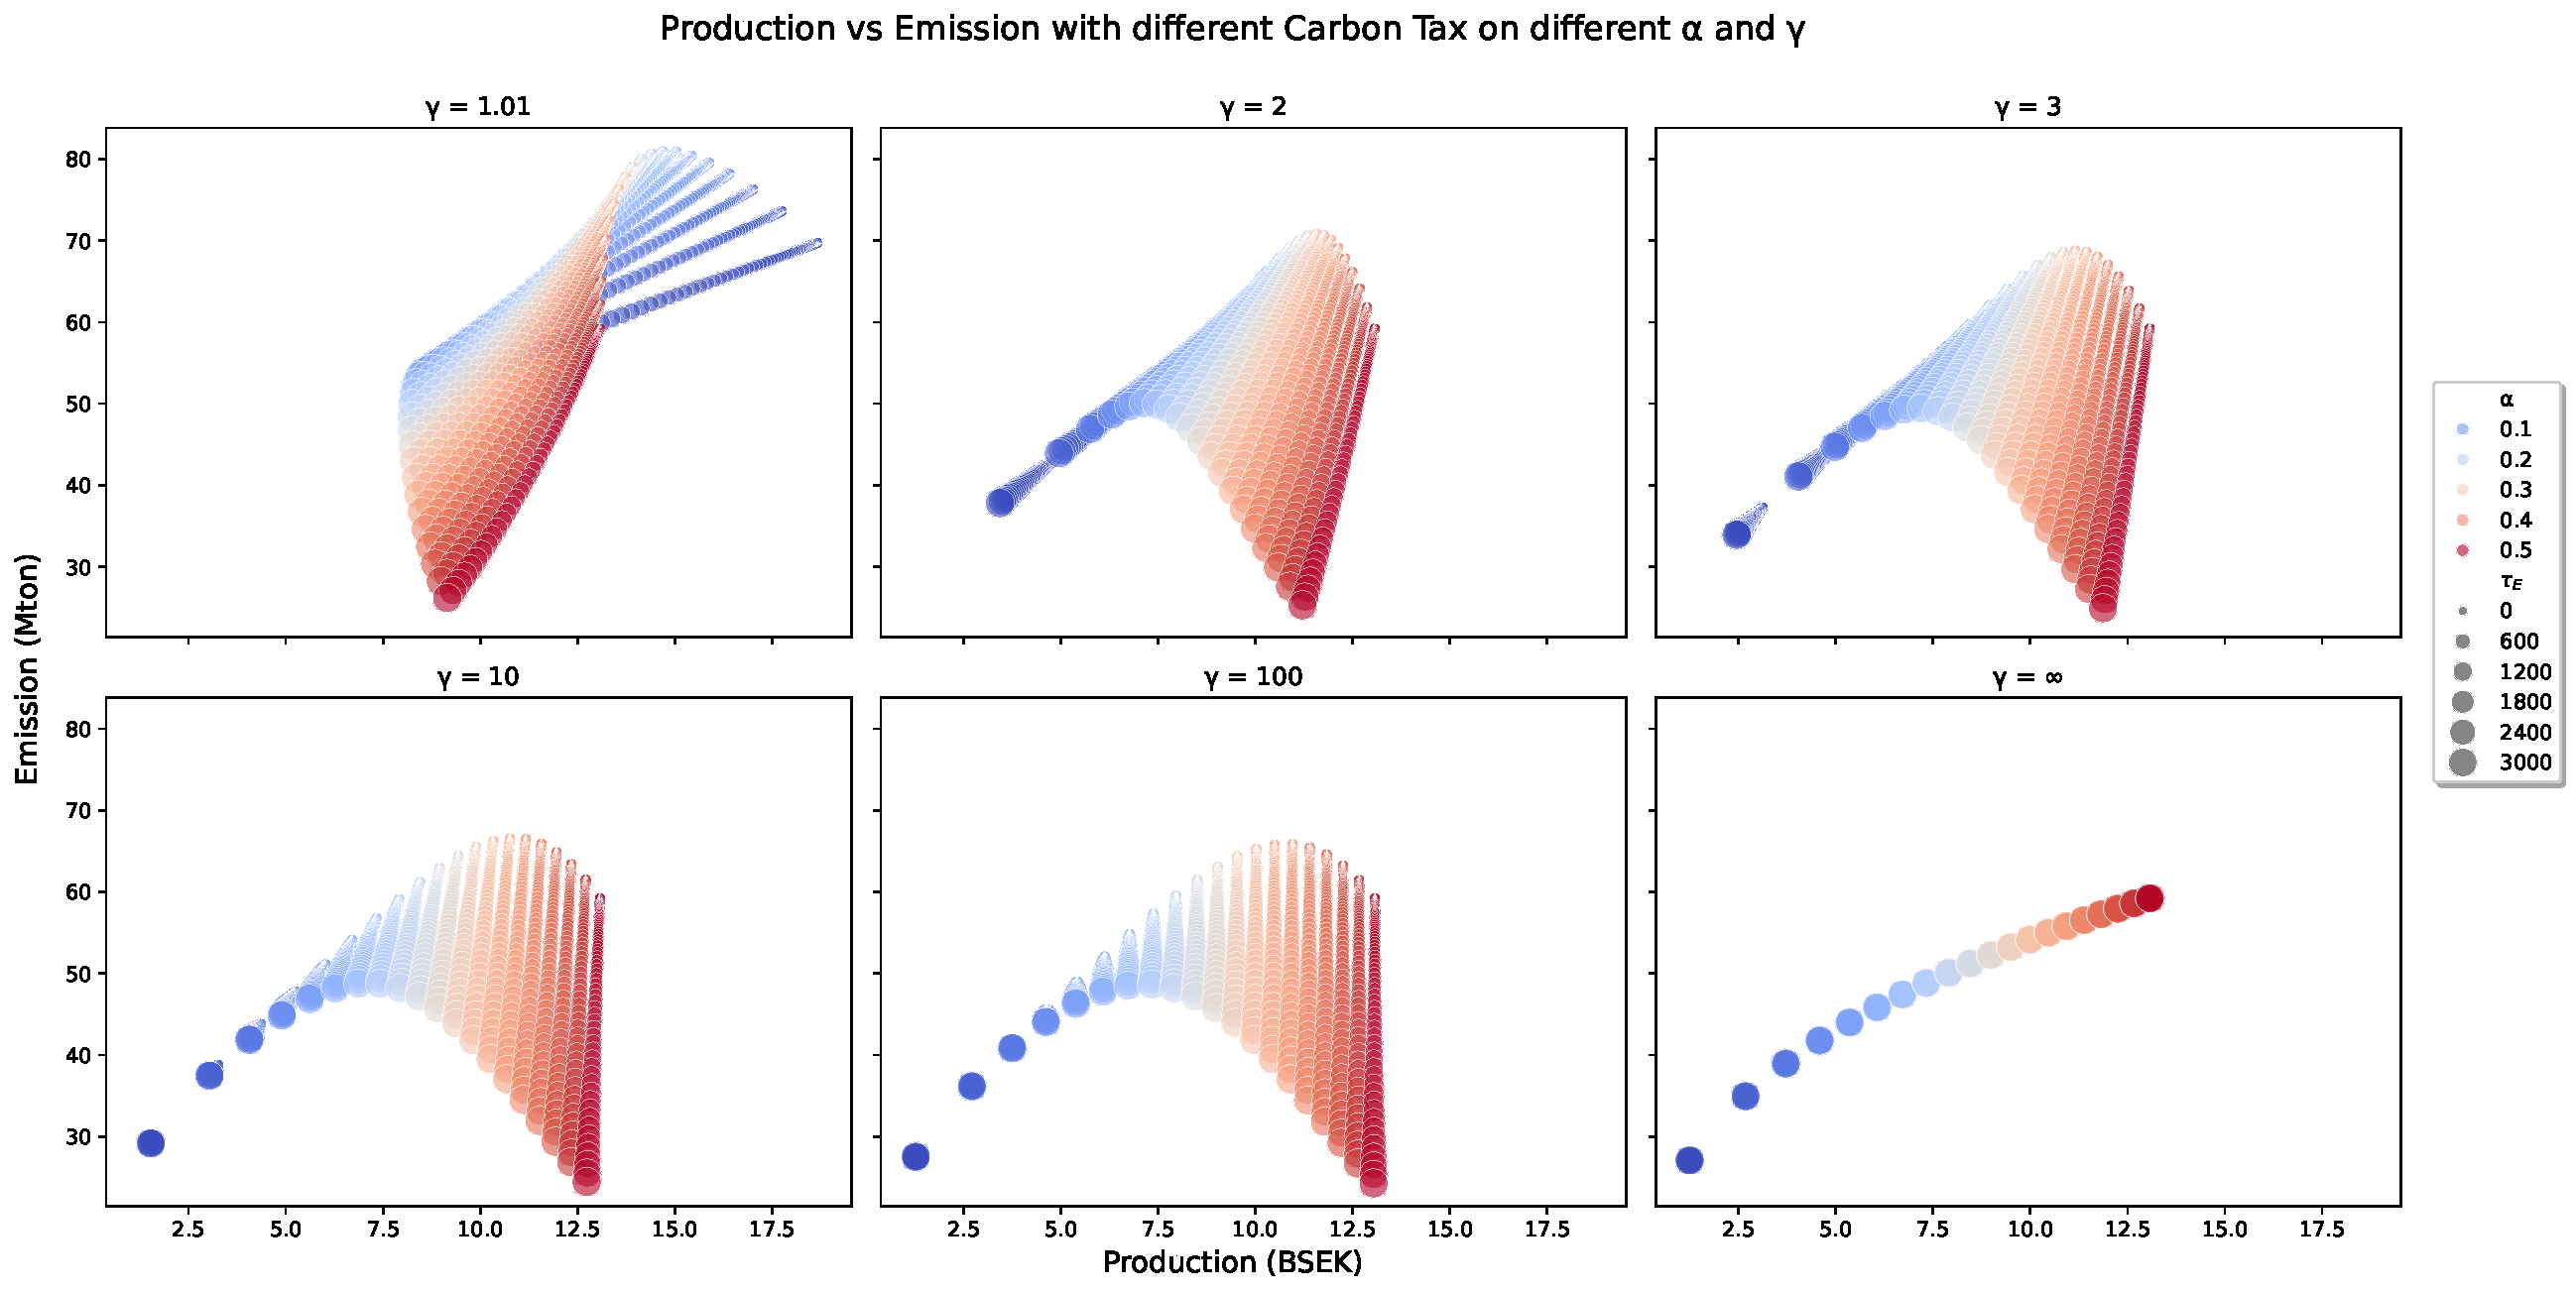
\includegraphics[width=7in]{Figures/production_emission.pdf}}
\caption{{\bf Relationship Between Production and Emissions: Impact of $\alpha$ and $\gamma$ on model's results.} This figure shows the impact of the $\alpha$ and $\gamma$ parameters on the relationship between production and emissions.}
\label{fig:production_emission}
\end{figure}
\vfill



\vfill
\begin{figure}[!htb]
\centerline{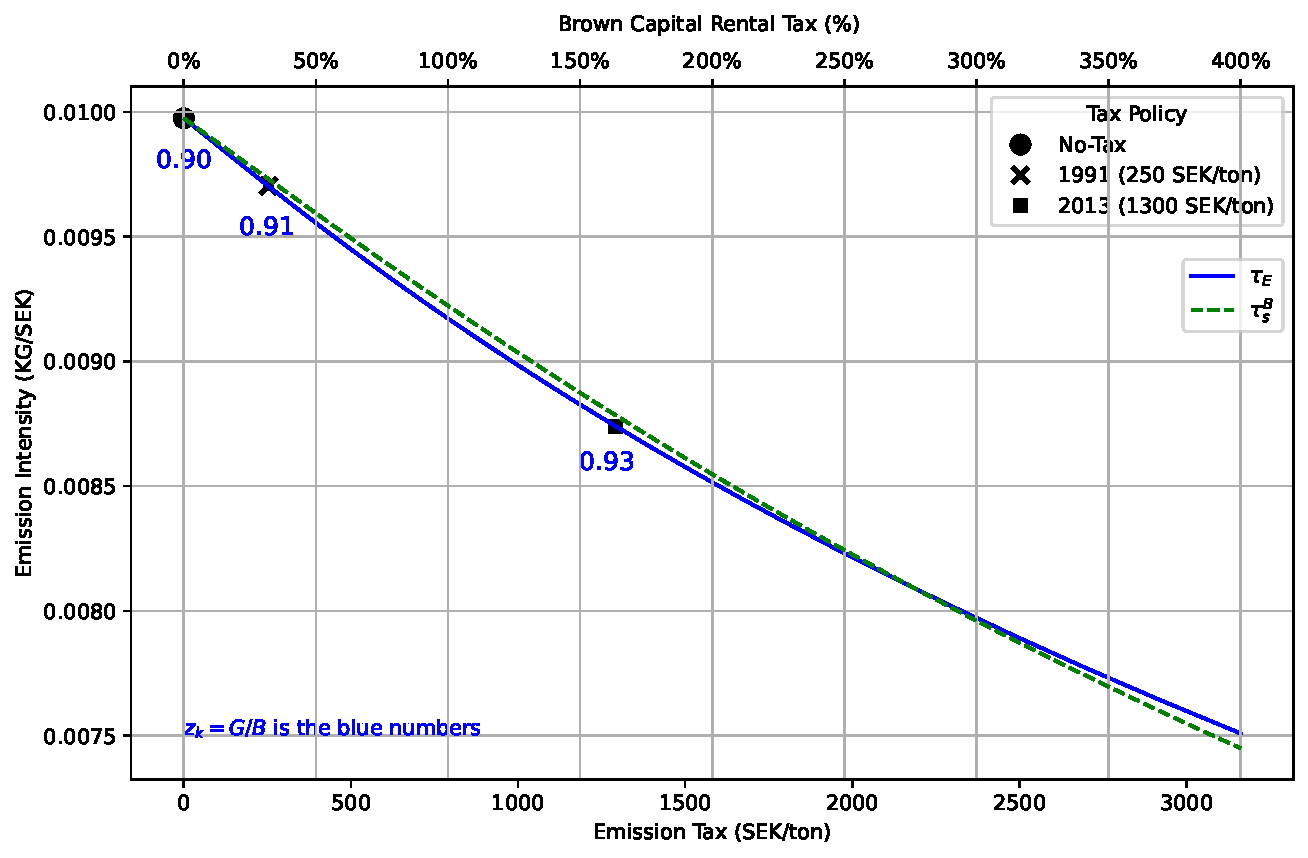
\includegraphics[width=7in]{Figures/intensity_tax_premium.pdf}}
\caption{{\bf Comparative Effectiveness of Carbon Tax, Green Subsidy, and Brown Tax on Carbon Intensity.} This figure quantifies the impact of different environmental policies on the carbon intensity of the economy.} \label{fig:intensity_tax_premium}
\end{figure}
\vfill

\vfill
\begin{figure}[!htb]
\centerline{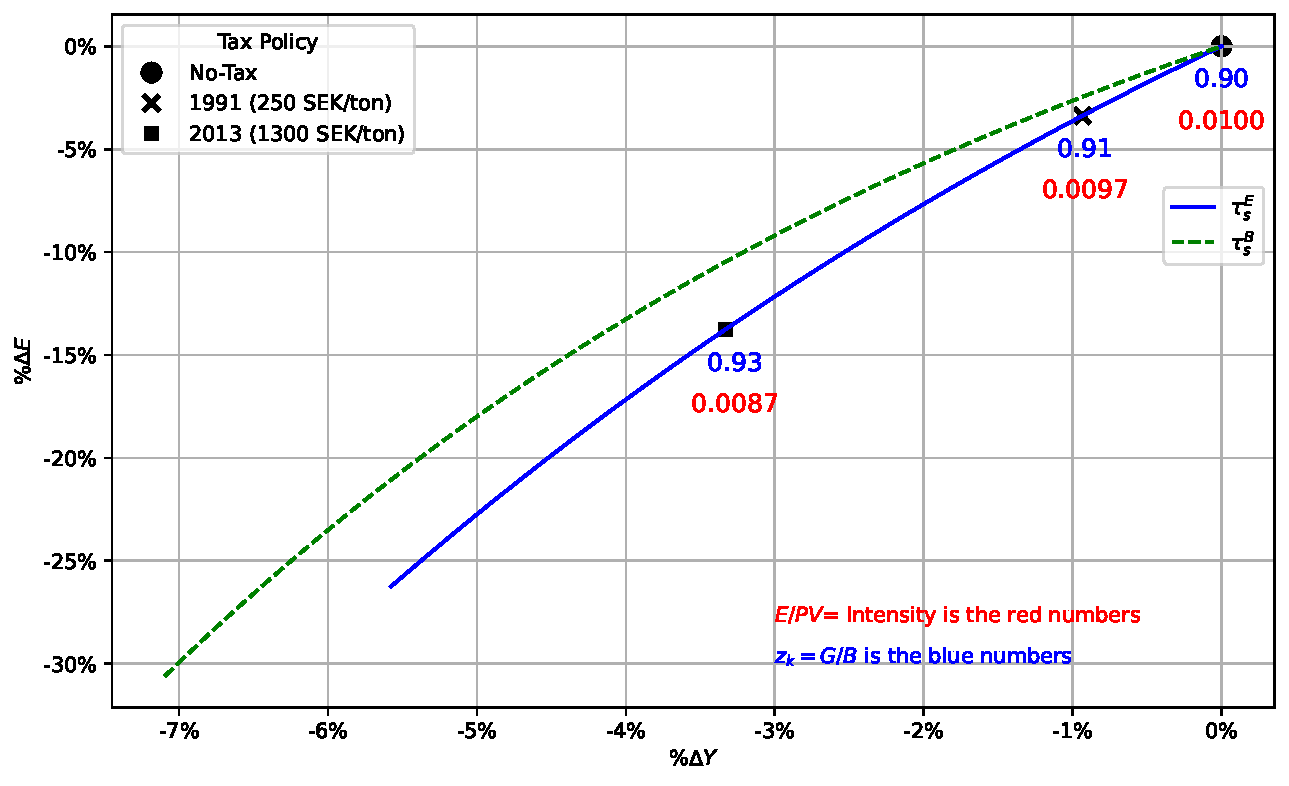
\includegraphics[width=7in]{Figures/emission_production.pdf}}
\caption{{\bf Comparative Effectiveness of Carbon Tax, Green Subsidy, and Brown Tax on Carbon Intensity.} This figure quantifies the impact of different environmental policies on the total emission and total production in the economy.} \label{fig:emission_production}
\end{figure}
\vfill


\end{document}
